\thispagestyle{toancuabinone}
\pagestyle{toancuabi}
\everymath{\color{toancuabi}}
%\blfootnote{$^1$\color{toancuabi}...}
\graphicspath{{../toancuabi/pic/}}
\begingroup
\AddToShipoutPicture*{\put(0,616){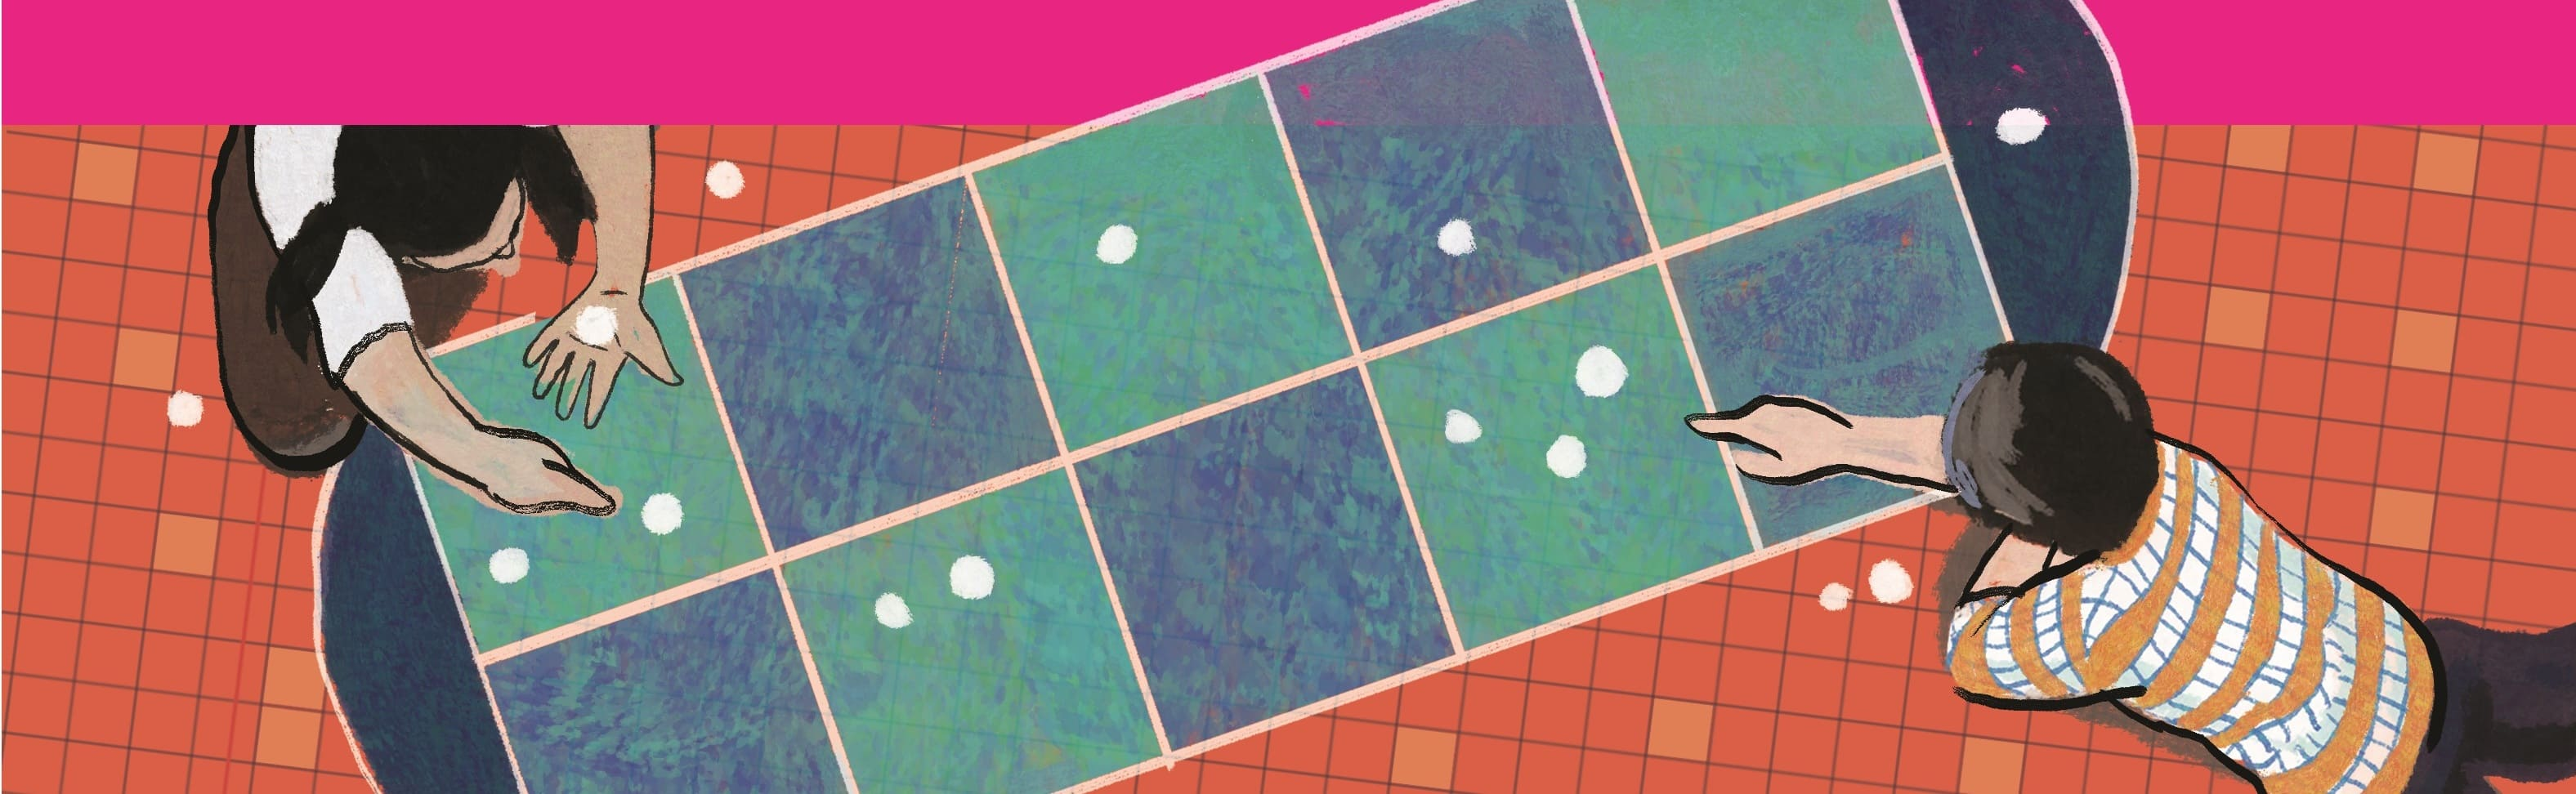
\includegraphics[width=19.3cm]{../bannertoancuabi}}}  
\AddToShipoutPicture*{\put(112,555){\includegraphics[scale=1]{../td.pdf}}} 
\centering
\endgroup
\vspace*{155pt}

\tikzset{
	pics/carc/.style args={#1:#2:#3}{
		code={
			\draw[pic actions] (#1:#3) arc(#1:#2:#3);
		}
	}
}
\begin{multicols}{2}
	Chắc không bạn nhỏ nào xa lạ với con xúc xắc đúng không? Những con xúc xắc đã gắn liền với tuổi thơ của chúng ta qua những trò chơi vô cùng thân quen mà hấp dẫn. Trong số này của Pi, mình cùng thảo luận về những câu đố liên quan tới dạng $3D$ của con xúc xắc. Đây là một trong những câu hỏi dạng lập luận không dùng lời văn phổ biến tại các kỳ thi, cũng như trong sách đố vui. Những câu đố dạng này cho ta biết một số góc nhìn của xúc xắc và yêu cầu xác định các mặt của~nó.
	\vskip 0.1cm
	Trong các bài toán này các mặt của con xúc xắc có thể được phân biệt bởi các số, các chấm, màu sắc hay biểu tượng trên chúng. Tuy nhiên phương pháp giải quyết bài toán về cơ bản là như nhau.
	\vskip 0.1cm
	Con xúc xắc được đề cập đến ở đây là con xúc xắc tiêu chuẩn gồm $6$ mặt. Với một góc nhìn $3D$ cố định, chúng ta thường chỉ nhìn được nhiều nhất $3$ mặt của con xúc xắc, như vậy là sẽ có ít nhất $3$ mặt bị ẩn đi. Các ví dụ trong bài viết này sẽ xem xét một số bài toán thường gặp khi tìm những mặt ẩn của một con xúc xắc. Các bạn nhỏ có thể nhận thấy ngay những ``mặt ẩn" sẽ thành ``mặt hiện" khi chúng ta chỉ ra được những cặp mặt đối diện của con xúc xắc. 
	\vskip 0.1cm
	Chúng ra bắt đầu với một ví dụ đơn giản khi đã biết $3$ góc nhìn của một con xúc xắc. 
	\vskip 0.1cm
	\textbf{\color{toancuabi}Ví dụ} $\pmb{1.}$ Tìm những cặp mặt đối diện của con xúc xắc biết rằng ta có ba góc nhìn trong hình dưới đây (các số tượng trưng cho số chấm trên mỗi mặt xúc xắc).
	\begin{figure}[H]
		\vspace*{-5pt}
		\centering
		\captionsetup{labelformat= empty, justification=centering}
		\includegraphics[width= 0.9\linewidth]{Pi5_xucxac_hinh1}
		\caption{\small\textit{\color{toancuabi}Hình $1$.}}
		\vspace*{-10pt}
	\end{figure}
	\textbf{\color{toancuabi}Lời giải.} Nhận thấy mặt $1$ xuất hiện nhiều nhất (ba lần) nên ta bắt đầu phân tích với mặt $1$. Ta có mặt $1$ kề với $4$ mặt: $2$, $3$, $4$ và $6$. Từ đó mặt đối diện với mặt $1$ là mặt $5$.
	\vskip 0.1cm
	Tiếp đến ta xét đến mặt $2$ (xuất hiện $2$ lần). Mặt $2$ kề với mặt $1$, $3$ và $6$. Do mặt $2$ không đối diện với mặt $5$ nên mặt đối diện của $2$ là mặt $4$. Như vậy mặt đối diện với mặt $3$ là mặt~$6$.
	\begin{table}[H]
		\vspace*{-5pt}
		\centering
		\setlength{\tabcolsep}{10pt}
		\renewcommand{\arraystretch}{1.2}
		\begin{tabular}{|l|c|c|c|}
			\hline
			Mặt	&$1$&	$2$&	$3$\\
			\hline
			Mặt đối diện&	$5$	&$4$&	$6$\\
			\hline
		\end{tabular}
	\vspace*{-5pt}
	\end{table}
	Như vậy ta đã tìm được tất cả các cặp mặt đối diện của con xúc xắc và từ đó tìm được những mặt ẩn đi trong mỗi góc nhìn.
	\vskip 0.1cm
	Các mặt của con xúc xắc mà chúng ta chơi thường được biểu thị bằng các con số hoặc chấm như Ví dụ $1$. Tuy nhiên, trong nhiều câu đố, các mặt có thể là các chữ cái, màu sắc hoặc ký hiệu. Ví dụ sau xét một trường hợp như vậy, tuy nhiên các bạn nhỏ sẽ thấy việc lập luận để tìm ra câu trả lời không có gì khác so với ví dụ trên.
	\vskip 0.1cm
	\textbf{\color{toancuabi}Ví dụ} $\pmb{2.}$ Đây là ba góc nhìn khác nhau của cùng một quân xúc xắc được tô bởi $6$ màu: {\color{red}Đỏ}, {\color{green}Xanh lá cây}, {\color{blue}Xanh da trời}, {\color{yellow}Vàng}, {\color{gocco}Tím} và {\color{toancuabi}Hồng} được biểu thị qua từ chỉ tên màu. Màu nào nằm trên mặt đối diện với mặt có màu ``Xanh da trời"?
	\begin{figure}[H]
		\vspace*{-5pt}
		\centering
		\captionsetup{labelformat= empty, justification=centering}
		\includegraphics[width= 1\linewidth]{Pi5_xucxac_Hinh2_New}
		\caption{\small\textit{\color{toancuabi}Hình $2$.}}
		\vspace*{-10pt}
	\end{figure}
	\textbf{\color{toancuabi}Lời giải.} Tương tự như Ví dụ $1$, ta bắt đầu phân tích từ mặt xuất hiện nhiều nhất là {\color{red}Đỏ}. Mặt {\color{red}Đỏ} kề với $4$ mặt: {\color{green}Xanh lá cây}, {\color{yellow}Vàng}, {\color{blue}Xanh da trời} và {\color{gocco}Tím}. Do đó, mặt đối diện với {\color{red}Đỏ} là {\color{toancuabi}Hồng}. Ta lại thấy mặt {\color{blue}Xanh da trời} kề với $3$ mặt: {\color{red}Đỏ}, {\color{green}Xanh lá cây}, {\color{gocco}Tím} và mặt {\color{blue}Xanh da trời} không đối diện với mặt {\color{toancuabi}Hồng}. Từ đó mặt {\color{blue}Xanh da trời} đối diện với mặt {\color{yellow}Vàng}.
	\begin{table}[H]
		\vspace*{-5pt}
		\centering
		\setlength{\tabcolsep}{7pt}
		\renewcommand{\arraystretch}{1.2}
		\begin{tabular}{|l|c|c|c|}
			\hline
			Mặt	& {\color{red}Đỏ}&	\makecell{\color{blue}Xanh\\ \color{blue}da trời}&	\makecell{\color{green}Xanh\\\color{green} lá cây}\\
			\hline
			Mặt đối diện&	{\color{toancuabi}Hồng}	&{\color{yellow}Vàng}&	{\color{gocco}Tím}\\
			\hline
		\end{tabular}
		\vspace*{-5pt}
	\end{table}
	Khi chúng ta có nhiều góc nhìn khác nhau của một con xúc xắc thì việc tìm những mặt ẩn của con xúc xắc cũng không có nhiều khó khăn phải không các bạn? Các bạn nhỏ hãy luyện tập thêm qua ví dụ sau nhé.
	\vskip 0.1cm
	\textbf{\color{toancuabi}Bài tập} $\pmb{1.}$ Bốn góc nhìn của một khối lập phương được cho ở hình bên dưới đây. Ký hiệu nào đối diện với $\Delta$?
	\begin{figure}[H]
		\vspace*{-5pt}
		\centering
		\captionsetup{labelformat= empty, justification=centering}
		\includegraphics[width= 1\linewidth]{Pi5_xucxac_hinh3}
		\caption{\small\textit{\color{toancuabi}Hình $3$.}}
		\vspace*{-10pt}
	\end{figure}
	Khi số góc nhìn của con xúc xắc giảm đi, chẳng hạn là hai góc nhìn như trong Ví dụ~$3$ thì việc tìm ra những cặp mặt đối diện của con xúc xắc trở nên khó khăn hơn. 
	\vskip 0.1cm
	\textbf{\color{toancuabi}Ví dụ} $\pmb{3.}$ Tìm những cặp mặt đối diện của quân xúc xắc biết hai góc nhìn sau.
	\begin{figure}[H]
		\vspace*{5pt}
		\centering
		\captionsetup{labelformat= empty, justification=centering}
		\includegraphics[width= 0.75\linewidth]{Pi5_xucxac_hinh4}
		\caption{\small\textit{\color{toancuabi}Hình $4$.}}
		\vspace*{-10pt}
	\end{figure}
	Để giải quyết bài toán ta cần tìm hiểu thêm tính chất của con xúc xắc và tìm cách mô tả nó một cách trực quan hơn. Về mặt hình học, con xúc xắc là khối lập phương -- gồm sáu mặt vuông và mười hai cạnh.  Tìm hiểu thêm một chút nữa, ta thấy khối lập phương có những tính chất sau.
	\vskip 0.1cm
	\textbf{\color{toancuabi}Tính chất $\pmb{1}$:} Mỗi mặt vuông trong khối lập phương kề với bốn mặt khác dọc theo bốn cạnh của nó.   
	\vskip 0.1cm
	\textbf{\color{toancuabi}Tính chất $\pmb{2}$:} Các mặt đối diện của khối lập phương thì không kề với nhau. 
	\vskip 0.1cm
	\textbf{\color{toancuabi}Tính chất $\pmb{3}$:} Mỗi mặt chỉ có duy nhất một số (tức không tồn tại hai mặt có cùng một số).
	\vskip 0.1cm
	Bây giờ, để dễ hình dung, ta biểu diễn mỗi mặt là một nút và mỗi cạnh là đường nối hai nút liền kề. Chẳng hạn, một con xúc xắc có thể biểu diễn như sau.
	\begin{figure}[H]
		\vspace*{-5pt}
		\centering
		\captionsetup{labelformat= empty, justification=centering}
		\includegraphics[width= 1\linewidth]{Pi5_xucxac_hinh5}
		\caption{\small\textit{\color{toancuabi}Hình $5$.}}
		\vspace*{-10pt}
	\end{figure}
	Đây chính là mô hình đồ thị của con xúc xắc. Mỗi nút được kết nối với bốn nút khác thông qua bốn đường biểu diễn bốn cạnh. Ví dụ, nút $6$ biểu diễn mặt  liền kề với các mặt $2, 4 , 5$ và $3$. Nút $6$ không nối trực tiếp với nút $1$:  chúng là các mặt đối diện nhau.
	\vskip 0.1cm
	Một số bạn khi vẽ mô hình của con xúc xắc theo cách trên có thể băn khoăn tại sao các nút lại ở các vị trí như trên mà không phải ở vị trí khác. Để hiểu tại sao ta làm quen với khái niệm hướng đi theo ``chiều kim đồng hồ".
	\vskip 0.1cm
	\textbf{\color{toancuabi}Cùng chiều và ngược chiều kim đồng hồ}
	\vskip 0.1cm
	Hình sau minh họa cho chúng ta thế nào là hướng đi theo chiều kim đồng hồ và hướng đi ngược chiều kim đồng hồ.
	\begin{figure}[H]
		\vspace*{-5pt}
		\centering
		\captionsetup{labelformat= empty, justification=centering}
		\includegraphics[width= 1\linewidth]{Pi5_xucxac_hinh6}
		\caption{\small\textit{\color{toancuabi}Hình $6$.}}
		\vspace*{-15pt}
	\end{figure}
	\begin{figure}[H]
	\vspace*{-10pt}
	\centering
	\captionsetup{labelformat= empty, justification=centering}
	\includegraphics[width= 1\linewidth]{Pi5_xucxac_hinh8.1_8.2}
	\caption{\small\textit{\color{toancuabi}Hình $7$.}}
	\vspace*{-10pt}
	\end{figure}
	Chẳng hạn, các hướng đi từ $A$ sang $B$, từ $B$ sang $C$ và từ $C$ sang $A$ trong Hình $8.1$ là ngược chiều kim đồng hồ, còn trong Hình~$8.2$ là cùng chiều kim đồng hồ. 
	\begin{figure}[H]
		\vspace*{-5pt}
		\centering
		\captionsetup{labelformat= empty, justification=centering}
		\includegraphics[width= 1\linewidth]{Pi5_xucxac_hinh8}
		\caption{\small\textit{\color{toancuabi}Hình $8.1$ \hspace*{60pt} Hình $8.2$.}}
		\vspace*{-10pt}
	\end{figure}
	Với mô hình của con xúc xắc, lấy bất kỳ bộ ba nút $A, B, C$ sao cho $A$ nối với $B$, $B$ nối với $C$ và $C$ nối với $A$ theo chiều kim đồng hồ; chúng đại diện cho góc nhìn $3D$ nào đó của con xúc xắc. Lưu ý rằng hướng và chiều của các mũi tên là rất quan trọng, nó buộc phải khớp với hình vẽ.  
	\vskip 0.1cm
	Chẳng hạn ta xét đồ thị bên dưới. Ở đây nút $4$ nối liền với nút $5$, nút $5$ nối liền với nút $6$ và nút $6$ nối liền với nút $4$ theo chiều kim đồng hồ. Điều đó ứng với góc nhìn $3D$ gồm mặt $4$ ở trên, mặt $5$ bên phải và mặt $6$ phía trước.    
	\begin{figure}[H]
		\vspace*{-5pt}
		\centering
		\captionsetup{labelformat= empty, justification=centering}
		\includegraphics[width= 1\linewidth]{Pi5_xucxac_hinh9}
		\caption{\small\textit{\color{toancuabi}Hình $9$.}}
		\vspace*{-10pt}
	\end{figure}
	Bây giờ, vận dụng cách mô tả con xúc xắc qua mô hình đồ thị như trên, ta sẽ đi tìm lời giải cho Ví dụ $3$.
	\vskip 0.1cm
	\textbf{\color{toancuabi}Lời giải Ví dụ} $\pmb{3.}$
	\vskip 0.1cm
	Lời giải được đưa ra dựa vào việc xét tính thuận chiều kim đồng hồ của những bộ ba góc nhìn đã biết của con xúc xắc.
	\vskip 0.1cm
	Trước hết, ta lập luận từ mặt xuất hiện cả trong hai góc nhìn đã biết là mặt $4$. Nhận thấy mặt $4$ kề với các mặt $1, 5, 3$ và $6$ nên ta có thể lập mô hình cho mặt $4$ và các mặt kề như sau. 
	\begin{figure}[H]
		\vspace*{-5pt}
		\centering
		\captionsetup{labelformat= empty, justification=centering}
		\includegraphics[width= 0.65\linewidth]{Pi5_xucxac_hinh10}
		\caption{\small\textit{\color{toancuabi}Hình $10$.}}
		\vspace*{-10pt}
	\end{figure}
	Mục tiêu bây giờ là ta phải điền các mặt $1, 3, 5, 6$ vào vị trí thích hợp.
	\vskip 0.1cm
	Từ góc nhìn đầu tiên ta có $4\to 5 \to 1$ theo chiều kim đồng hồ nên ta điền mặt $5$ và $1$ như hình dưới đây.
	\begin{figure}[H]
		\vspace*{-5pt}
		\centering
		\captionsetup{labelformat= empty, justification=centering}
		\includegraphics[width= 0.93\linewidth]{Pi5_xucxac_hinh11}
		\caption{\small\textit{\color{toancuabi}Hình $11$.}}
		\vspace*{-10pt}
	\end{figure}
	Tương tự, từ góc nhìn thứ hai ta có $4 \to 3 \to 6$ theo chiều kim đồng hồ nên ta thu được 
	\begin{figure}[H]
		\vspace*{-5pt}
		\centering
		\captionsetup{labelformat= empty, justification=centering}
		\includegraphics[width= 0.93\linewidth]{Pi5_xucxac_hinh12}
		\caption{\small\textit{\color{toancuabi}Hình $12$.}}
		\vspace*{-10pt}
	\end{figure}
	Từ đây ta suy ra mặt đối diện với $1$ là $6$, mặt đối diện với $3$ là $5$ và tất nhiên mặt đối diện với $4$ là $2$.
	\vskip 0.1cm
	\begin{table}[H]
		\vspace*{-5pt}
		\centering
		\setlength{\tabcolsep}{10pt}
		\renewcommand{\arraystretch}{1.2}
		\begin{tabular}{|l|c|c|c|}
			\hline
			Mặt& 	$1$&	$2$&	$3$\\
			\hline
			Mặt đối diện&	$6$&	$4$&	$5$\\
			\hline
		\end{tabular}
		\vspace*{-5pt}
	\end{table}
	Lưu ý là khi biểu diễn góc nhìn thứ nhất lên mô hình, ta cũng có thể điền như sau
	\begin{figure}[H]
		\vspace*{-5pt}
		\centering
		\captionsetup{labelformat= empty, justification=centering}
		\includegraphics[width= 0.65\linewidth]{Pi5_xucxac_hinh13}
		\caption{\small\textit{\color{toancuabi}Hình $13$.}}
		\vspace*{-5pt}
	\end{figure}
	Và khi đó góc nhìn thứ hai được điền tiếp vào mô hình là
	\begin{figure}[H]
		\vspace*{-5pt}
		\centering
		\captionsetup{labelformat= empty, justification=centering}
		\includegraphics[width= 0.65\linewidth]{Pi5_xucxac_hinh14}
		\caption{\small\textit{\color{toancuabi}Hình $14$.}}
		\vspace*{-10pt}
	\end{figure}
	Nhưng các em có thể thấy đây là hai cách biểu diễn như nhau và cùng suy ra được kết quả giống nhau về mặt đối diện của con xúc xắc.
	\vskip 0.1cm
	Biểu diễn con xúc xắc theo kiểu ``mô hình đồ thị" thật là hay đúng không? Chỉ bằng một vài bước biểu diễn những góc nhìn sẵn có là ta có thể tìm ra những mặt ẩn của con xúc xắc một cách chính xác. Các em hãy luyện tập thêm phương pháp này để làm bài tập sau nhé.
	\vskip 0.1cm
	\textbf{\color{toancuabi}Bài tập} $\pmb{2.}$ Đây là hai góc nhìn khác nhau của một con xúc xắc. Giả sử dưới đáy có hai chấm thì số chấm ở trên cùng của con xúc xắc là bao nhiêu?
	\begin{figure}[H]
		\vspace*{-5pt}
		\centering
		\captionsetup{labelformat= empty, justification=centering}
		\includegraphics[width= 0.7\linewidth]{Pi5_xucxac_hinh15}
		\caption{\small\textit{\color{toancuabi}Hình $15$.}}
		\vspace*{-10pt}
	\end{figure}
	Dưới đây ta xét thêm một số ví dụ khác nữa để xem kỹ thuật trên được vận dụng như thế nào cho những tình huống khác nhau. 
	\vskip 0.1cm
	\textbf{\color{toancuabi}Xúc xắc dạng phẳng}
	\vskip 0.1cm
	Bên cạnh dạng $3D$ của con xúc xắc, dạng $2D$ -- dạng phẳng cũng hay được sử dụng. Thử thách đặt ra cho chúng ta là nếu ta biết dạng phẳng của con xúc xắc thì có thể tìm xem một dạng $3D$ được đưa ra có phù hợp hay không phù hợp. Với thử thách này, chúng ta tiếp tục dùng cách mô hình hóa con xúc xắc để tìm lời giải. Cách làm được minh họa qua ví dụ dưới~đây.
	\vskip 0.1cm
	\textbf{\color{toancuabi}Ví dụ} $\pmb{4.}$ Cho một con xúc xắc có dạng phẳng như sau.
	\begin{figure}[H]
		\vspace*{-5pt}
		\centering
		\captionsetup{labelformat= empty, justification=centering}
		\includegraphics[width= 0.9\linewidth]{Pi5_xucxac_hinh16}
		\vspace*{-15pt}
	\end{figure}
	Dạng $3D$ nào dưới đây không phù hợp với nó?
	 \begin{figure}[H]
	 	\vspace*{-5pt}
	 	\centering
	 	\captionsetup{labelformat= empty, justification=centering}
	 	\includegraphics[width= 0.9\linewidth]{Pi5_xucxac_hinh16.1}
	 	\caption{\small\textit{\color{toancuabi}Hình $16$.}}
	 	\vspace*{-10pt}
	 \end{figure}
	Để giải quyết Ví dụ $4$, ta giới thiệu một nhận xét rất hữu ích sau khi xem xét về chiều của những bộ ba có mặt đối diện với nhau.
	\vskip 0.1cm
	-- \textbf{\color{toancuabi}Nhận xét.}  Với mỗi bộ ba có cùng hai mặt bên kề nhau, chiều của bộ ba có ``mặt trên" sẽ là ngược với chiều của bộ ba ``mặt dưới". Cụ thể là, nếu bộ ba $(A, B, C)$ có $A \to B \to C$ cùng chiều kim đồng hồ, mặt $B'$ đối diện với mặt $B$ thì $A \to B' \to C$ là ngược chiều kim đồng hồ.
	\begin{figure}[H]
		\vspace*{-5pt}
		\centering
		\captionsetup{labelformat= empty, justification=centering}
		\includegraphics[width= 1\linewidth]{Pi5_xucxac_hinh17}
		\caption{\small\textit{\color{toancuabi}Hình $17$.}}
		\vspace*{-10pt}
	\end{figure}
	\textbf{\color{toancuabi}Lời giải.} 
	Trước hết, ta cần tìm mô hình đồ thị của con xúc xắc. Nhận thấy mặt ``mặt trời" \includegraphics[scale=0.05]{Pi5_xucxac_mattroi} kề với các mặt ``đám mây"   \includegraphics[scale=0.05]{Pi5_xucxac_dammay}, ``ngôi sao" \includegraphics[scale=0.05]{Pi5_xucxac_sao} , ``mặt trăng" \includegraphics[scale=0.05]{Pi5_xucxac_mattrang}  và ``kim cương" \includegraphics[scale=0.09]{Pi5_xucxac_kimcuong} nên ta có biểu diễn dưới đây.
	\begin{figure}[H]
%		\vspace*{-5pt}
		\centering
		\captionsetup{labelformat= empty, justification=centering}
		\includegraphics[width= 0.63\linewidth]{Pi5_xucxac_hinh18}
		\caption{\small\textit{\color{toancuabi}Hình $18$.}}
		\vspace*{-10pt}
	\end{figure}
	Nhận thấy mặt đối diện với ``mặt trời" là mặt ``tam giác"   và theo nhận xét ở trên, khi cùng chung hai mặt kề thì các bộ ba có ``mặt trời" và ``tam giác" tương ứng sẽ ngược chiều với nhau.
	\begin{figure}[H]
		\vspace*{-5pt}
		\centering
		\captionsetup{labelformat= empty, justification=centering}
		\includegraphics[width= 0.63\linewidth]{Pi5_xucxac_hinh19}
		\caption{\small\textit{\color{toancuabi}Hình $19$.}}
		\vspace*{-10pt}
	\end{figure}
	Tiếp theo đó, ta biểu diễn dạng $3D$ của từng quân xúc xắc $A, B, C$ và $D$ thành mô hình đồ thị. Nếu có hình không thỏa mãn đồ thị của con xúc xắc đã cho thì đó chính là đáp án.
	\vskip 0.1cm
	Bước $1$: Ở lựa chọn $A$ ta thấy góc nhìn biểu diễn  \includegraphics[scale=0.05]{Pi5_xucxac_tamgiac} $\to$ \includegraphics[scale=0.05]{Pi5_xucxac_dammay} $\to$
	\includegraphics[scale=0.05]{Pi5_xucxac_sao}  đi theo chiều kim đồng hồ. Kết quả này là phù hợp vì biểu diễn tương ứng  \includegraphics[scale=0.05]{Pi5_xucxac_mattroi} $\to$ \includegraphics[scale=0.05]{Pi5_xucxac_dammay} $\to$
	\includegraphics[scale=0.05]{Pi5_xucxac_sao}   là ngược chiều kim đồng hồ.
	\begin{figure}[H]
		\vspace*{-5pt}
		\centering
		\captionsetup{labelformat= empty, justification=centering}
		\includegraphics[width= 0.93\linewidth]{Pi5_xucxac_hinh20}
		\caption{\small\textit{\color{toancuabi}Hình $20$.}}
		\vspace*{-5pt}
	\end{figure}
	Vậy $A$ là phù hợp.
	\vskip 0.1cm
	Bước $2$: Ở lựa chọn $B$ ta thấy góc nhìn khi biểu diễn  \includegraphics[scale=0.05]{Pi5_xucxac_mattroi} $\to$ \includegraphics[scale=0.05]{Pi5_xucxac_mattrang} $\to$
	\includegraphics[scale=0.05]{Pi5_xucxac_sao}   đi theo chiều kim đồng hồ, phù hợp với tính thuận chiều trong mô hình biểu diễn.
	\begin{figure}[H]
		\vspace*{-5pt}
		\centering
		\captionsetup{labelformat= empty, justification=centering}
		\includegraphics[width= 0.95\linewidth]{Pi5_xucxac_hinh21}
		\caption{\small\textit{\color{toancuabi}Hình $21$.}}
		\vspace*{-10pt}
	\end{figure}
	Vậy $B$ là phù hợp.
	\vskip 0.1cm
	Bước $3$: Ở lựa chọn $C$ ta thấy góc nhìn biểu diễn  \includegraphics[scale=0.05]{Pi5_xucxac_mattroi} $\to$ \includegraphics[scale=0.05]{Pi5_xucxac_sao} $\to$
	\includegraphics[scale=0.05]{Pi5_xucxac_dammay} cùng chiều kim đồng hồ, phù hợp với tính thuận chiều trong mô hình biểu diễn.
	\begin{figure}[H]
		\vspace*{-5pt}
		\centering
		\captionsetup{labelformat= empty, justification=centering}
		\includegraphics[width= 0.95\linewidth]{Pi5_xucxac_hinh22}
		\caption{\small\textit{\color{toancuabi}Hình $22$.}}
		\vspace*{-10pt}
	\end{figure}
	Vậy $C$ là phù hợp.
	\begin{figure}[H]
		\vspace*{-5pt}
		\centering
		\captionsetup{labelformat= empty, justification=centering}
		\includegraphics[width= 0.95\linewidth]{Pi5_xucxac_hinh23}
		\caption{\small\textit{\color{toancuabi}Hình $23$.}}
		\vspace*{-5pt}
	\end{figure}
	Bước $4$: Ở lựa chọn $D$ ta thấy biểu diễn \includegraphics[scale=0.05]{Pi5_xucxac_tamgiac} $\to$ \includegraphics[scale=0.05]{Pi5_xucxac_dammay} $\to$
	\includegraphics[scale=0.09]{Pi5_xucxac_kimcuong} đi cùng chiều kim đồng hồ, điều này mâu thuẫn với trong biểu diễn của mô hình \includegraphics[scale=0.05]{Pi5_xucxac_mattroi} $\to$ \includegraphics[scale=0.05]{Pi5_xucxac_dammay} $\to$
	\includegraphics[scale=0.09]{Pi5_xucxac_kimcuong}  cũng cùng chiều kim đồng hồ.
	\vskip 0.1cm
	Vậy $D$ là không phù hợp.
	\vskip 0.1cm
	Từ các bước trên ta thấy rằng chỉ có dạng $3D$ của con xúc xắc $D$ là không phù hợp. Và đó chính là đáp án.
	\vskip 0.1cm
	Dưới đây là một bài tập để các em luyện tập thêm về tìm con xúc xắc không phù hợp với dạng phẳng của con xúc xắc.
	\vskip 0.1cm
	\textbf{\color{toancuabi}Bài tập} $\pmb{3.}$ Con xúc xắc nào dưới đây có thể được gấp lại từ tấm bìa bên dưới?
	\begin{figure}[H]
		\vspace*{-5pt}
		\centering
		\captionsetup{labelformat= empty, justification=centering}
		\includegraphics[width= 0.7\linewidth]{Pi5_xucxac_hinh24_1}
		\includegraphics[width= 1\linewidth]{Pi5_xucxac_hinh24_2}
		\caption{\small\textit{\color{toancuabi}Hình $24$.}}
		\vspace*{-10pt}
	\end{figure}
	Các em thân mến, bài viết này giới thiệu đến các em một cách để tìm ra những mặt ẩn của con xúc xắc. Đây là một kỹ thuật rất hữu ích đúng không nào, các em hãy luyện tập và áp dụng để tìm ra lời giải trong những tình huống tương tự về con xúc xắc mà mình gặp. Liên quan đến con xúc xắc còn nhiều những câu đố thú vị, các độc giả của Pi thấy có những câu đố hay khác thì hãy gửi bài để chia sẻ cùng Pi nhé.   
	\vskip 0.1cm
	\textbf{\color{toancuabi}Tài liệu tham khảo.}
	Kiran Ananthpur Bacche, \textit{Mathematical Approach to Puzzle Solving}, Notion Press $2016$.	
\end{multicols}
\newpage
\begingroup
\AddToShipoutPicture*{\put(165,680){\includegraphics[scale=1]{../tieude.pdf}}} 
\centering
\endgroup
\vspace*{25pt}

\begin{multicols}{2}
	Thám tử Xuân Phong và Thanh tra Lê Kính được mời tới sở cảnh sát để thẩm vấn những người tình nghi trong một vụ án kỳ lạ. Thủ phạm một vụ lừa đảo cửa hàng máy tính là một trong số $8$ người bạn thân thiết của nhau. Khi được hỏi riêng từng người, ai cũng phủ nhận việc mình tham gia vào vụ phạm pháp. Thanh tra Lê Kính nói trước với Xuân Phong: ``Anh Phong biết không, ai trong số $8$ người này cũng đều nắm rõ công việc của những người còn lại, tuy nhiên vì thân thiết nhau quá nên ngại không dám nêu tên kẻ lừa đảo~ra."
	\vskip 0.1cm
	Thám tử Xuân Phong có thể tách ra một nhóm bất kỳ (có  ít nhất hai người) trong số $8$ người đó và đưa ra câu hỏi: ``Trong số các anh có ai là kẻ lừa đảo cửa hàng máy tính không?" Nếu trong nhóm đó không có kẻ lừa đảo cần tìm, thì tất cả đều trả lời ``Không", còn nếu trong trường hợp ngược lại, tất cả đều nói ``Có" (cả kẻ lừa đảo cũng trả lời ``Có", cố gắng hòa lẫn với những người xung quanh để không bị lộ).
	\begin{figure}[H]
		\vspace*{-5pt}
		\centering
		\captionsetup{labelformat= empty, justification=centering}
		\includegraphics[width= 1\linewidth]{xp}
		\vspace*{-15pt}
	\end{figure}
	Vậy Xuân Phong sẽ phải đưa ra ít nhất bao nhiêu câu hỏi để xác định chính xác kẻ phạm tội? Các em cùng giúp đỡ Xuân Phong và Lê Kính trong vụ điều tra này nhé.
\end{multicols}
\vspace*{-10pt}
\rule{1\linewidth}{0.1pt}
\begingroup
\AddToShipoutPicture*{\put(110,325){\includegraphics[scale=1]{../tieude11.pdf}}} 
\centering
\endgroup
\vspace*{40pt}

\begin{multicols}{2}
	$\pmb{1.}$ Trong một kỳ nghỉ hè, Tâm và Bảo cùng đi du lịch trên một chuyến tàu hỏa. Hai toa mà họ ngồi là các toa liền kề nhau. Toa tàu của Tâm là toa thứ $5$ tính từ đầu tàu, còn toa  của Bảo lại là toa thứ $7$ tính từ đuôi tàu. Hỏi đoàn tàu của hai bạn hôm đó có bao nhiêu toa?
	\begin{figure}[H]
		\vspace*{-5pt}
		\centering
		\captionsetup{labelformat= empty, justification=centering}
		\includegraphics[width= 1\linewidth]{b1}
		\vspace*{-15pt}
	\end{figure}
	$\pmb{2.}$	Có ba người bạn muốn đi ca nô vượt qua một con sông, chở theo một cái tủ lạnh. Chiếc ca nô chỉ đủ chỗ cho $2$ người và tủ lạnh, hoặc chỉ cho $3$ người. Nhưng rắc rối ở chỗ là cái tủ lạnh quá nặng, nên phải có cả sức $3$ người mới đủ để khiêng nó lên ca nô hoặc đẩy xuống khỏi ca nô. Hỏi họ có thể qua được sông hay không?
	\begin{figure}[H]
		\vspace*{-10pt}
		\centering
		\captionsetup{labelformat= empty, justification=centering}
		\includegraphics[width= 1\linewidth]{b2}
		\vspace*{-15pt}
	\end{figure}
	$\pmb{3.}$ Trong một vương quốc nọ các thần dân chia thành $2$ nhóm người: một nhóm Thật thà gồm toàn những người nói thật, và nhóm kia là Dối trá gồm toàn những người chỉ nói dối. Trong một buổi tối nọ, có $10$ người lần lượt bước vào một ngôi nhà, mỗi người trong số họ (trừ người cuối cùng) viết trên một mảnh giấy đặc biệt để thông báo người sẽ vào tiếp theo anh ta là Thật thà hay Dối trá. Nếu như tin vào những gì viết trên $9$ mảnh giấy đó, thì toàn là người Dối trá đã bước vào nhà. Hỏi trên thực tế có tất cả bao nhiêu người Dối trá đã tới ngôi nhà đó.	
		\begin{figure}[H]
		\vspace*{-5pt}
		\centering
		\captionsetup{labelformat= empty, justification=centering}
		\includegraphics[width= 1\linewidth]{b3}
		\vspace*{-15pt}
	\end{figure}
	$\pmb{4.}$ Hai chiếc máy bơm cùng nhau bơm đầy nước cho một bể bơi trong vòng $2$ giờ. Hỏi mỗi chiếc máy bơm sẽ bơm đầy bể trong bao nhiêu lâu, biết rằng thời gian bơm đầy của hai máy bơm tính theo giờ là các số nguyên khác nhau.
	\begin{figure}[H]
		\vspace*{-5pt}
		\centering
		\captionsetup{labelformat= empty, justification=centering}
		\includegraphics[width= 0.9\linewidth]{b4}
		\vspace*{-5pt}
	\end{figure}
	$\pmb{5.}$ Trên một hòn đảo nọ có các thổ dân sinh sống, một số người thì luôn nói thật, còn những người còn lại thì luôn nói dối. Một lần nọ, ba thổ dân là anh Tit, anh Te và anh Tu gặp nhau. Một người trong số họ nói ``Tit và Te -- cả hai đều là những  người nói dối'', một người khác nói ``Tit và Tu -- cả hai đều là những người nói dối" (tuy nhiên không rõ chính xác ai nói những câu này). Hỏi có bao nhiêu người nói dối trong số $3$ người này.
	\begin{figure}[H]
		\vspace*{-5pt}
		\centering
		\captionsetup{labelformat= empty, justification=centering}
		\includegraphics[width= 1\linewidth]{b5}
		\vspace*{-15pt}
	\end{figure}
	$\pmb{6.}$ Có $10$ cái hộp bút, mỗi hộp đựng một số chiếc bút chì màu, không có hộp nào là rỗng. Biết rằng số bút chì ở hai hộp bất kỳ là khác nhau, hơn nữa những chiếc bút chì trong mỗi hộp đều có màu khác nhau, em hãy chỉ ra là có thể nhặt ra từ mỗi chiếc hộp một chiếc bút để nhận được $10$ chiếc bút chì có màu hoàn toàn khác nhau. 
	\begin{figure}[H]
		\vspace*{-5pt}
		\centering
		\captionsetup{labelformat= empty, justification=centering}
		\includegraphics[width= 1\linewidth]{b6}
		\vspace*{-5pt}
	\end{figure}
\end{multicols}
\vspace*{-10pt}
\rule{1\linewidth}{0.1pt}
\begingroup
\AddToShipoutPicture*{\put(112,175){\includegraphics[scale=1]{../tieude2.pdf}}} 
\centering
\endgroup
\vspace*{70pt}

\begin{multicols}{2}
$\pmb{1.}$ Tuổi của An nhiều hơn tuổi của Bình là $3$. Tuổi của Nguyên nhân với tuổi của Bình    lớn hơn   tuổi của An nhân với tuổi của Bình là  $9$. Hỏi tuổi của An nhiều hơn tuổi của Nguyên là bao nhiêu?
\vskip 0.1cm
\textit{Lời giải.} Giả sử tuổi của An là $a$, tuổi của Nguyên là $b$. Khi đó tuổi của Bình là $a - 3$ $(a>3)$. Theo đề bài ta có
\begin{align*}
	b(a-3) = a(a-6)+9
\end{align*}
Từ đó ta có $(a-3)(a-b-3)=0$.
\vskip 0.1cm
Nhưng $a>3$, vì vậy $a-b=3$. Vậy An lớn hơn Nguyên $3$ tuổi.
\begin{figure}[H]
	\centering
	\vspace*{-5pt}
	\captionsetup{labelformat= empty, justification=centering}
	\includegraphics[width=1\linewidth]{b11}
	\vspace*{-15pt}
\end{figure}
$\pmb{2.}$ Một bộ gồm $19$ quả cân với các khối lượng $1$ g, $2$ g, ..., $19$ g. Có $9$ quả trong đó làm bằng sắt, $9$ quả làm từ đồng và $1$ quả làm bằng vàng. Tổng khối lượng các quả bằng sắt \linebreak chênh lệch so với tổng khối lượng các quả bằng đồng là $90$ g. Hỏi khối lượng của quả cân bằng vàng là bao nhiêu?
\begin{figure}[H]
	\centering
	\vspace*{-5pt}
	\captionsetup{labelformat= empty, justification=centering}
	\includegraphics[width=1\linewidth]{b22}
	\vspace*{-15pt}
\end{figure}
\textit{Lời giải.} Chênh lệch tổng khối lượng của các quả cân sắt so với  tổng khối lượng các quả cân đồng là $90$ g khi và chỉ khi $9$ quả trong nhóm nhẹ hơn có các khối lượng là $1, 2, \ldots, 9$ (g), trong khi $9$ quả trong nhóm nặng hơn là $11, 12, \ldots, 19$ (g). Suy ra quả cân bằng vàng có khối lượng là $10$ g.
\vskip 0.1cm
$\pmb{3.}$ Trong phiên chợ Tết, người ta bày trên bàn một mâm kẹo rất ngon để tặng các bạn nhỏ đến chợ. Bạn nhỏ đầu tiên lấy $1/10$ tổng số kẹo. Bạn nhỏ thứ hai lấy $1/10$ tổng số kẹo còn lại và thêm cả $1/10$ số kẹo bạn thứ nhất đã lấy.  Bạn nhỏ thứ ba lấy $1/10$ tổng số kẹo còn lại trên bàn sau khi bạn thứ hai lấy kẹo và thêm cả $1/10$ số kẹo  các bạn trước đã lấy. Bạn nhỏ thứ tư lấy $1/10$ tổng số kẹo còn lại trên bàn sau khi bạn thứ ba lấy và thêm cả $1/10$ số kẹo các bạn trước đã lấy... Cứ như vậy cho đến khi trên bàn không còn cái kẹo nào. Hỏi có tất cả bao nhiêu bạn nhỏ đã đến lấy kẹo, và bạn nào lấy nhiều nhất trong số họ?
\begin{figure}[H]
	\centering
	\vspace*{-5pt}
	\captionsetup{labelformat= empty, justification=centering}
	\includegraphics[width=0.85\linewidth]{b33}
	\vspace*{-15pt}
\end{figure}
\textit{Lời giải.} Giả sử ban đầu trên bàn có $N$ cái kẹo. Giả sử một số bạn đầu tiên lấy đi mất $k$ chiếc kẹo. Khi đó trên bàn còn $(N-k)$ chiếc. Bạn tiếp theo sẽ lấy bao nhiêu kẹo? $1/10$ của số kẹo còn lại là $(N-k)/10$, còn $1/10$ số kẹo các bạn trước đã lấy là $k/10$. Vậy bạn tiếp theo sẽ lấy $N/10$ chiếc kẹo. Như vậy suy ra mỗi bạn nhỏ đều lấy cùng một số kẹo là $N/10$ không phụ thuộc vào thứ tự. Vì vào một thời điểm, số kẹo cũng cạn hết nên suy ra có tất cả $10$ bạn nhỏ đã đến lấy kẹo, hơn nữa bạn nào cũng lấy số kẹo như nhau, khỏi phải suy bì.
\vskip 0.1cm
$\pmb{4.}$ Bác Lan có một mảnh vải như trong hình vẽ
\begin{center}
	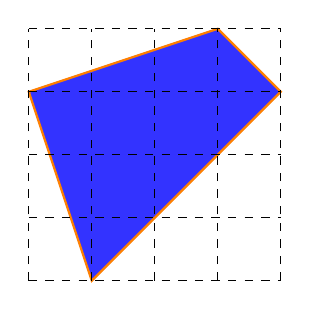
\begin{tikzpicture}[scale=0.8]
		\filldraw [color=blue!80] (1,0)--(4,3)--(3,4)--(0,3)--cycle;
		\draw [thick,orange]  (1,0)--(4,3)--(3,4)--(0,3)--cycle;
		\draw [dashed] (0,0) grid (4,4);
	\end{tikzpicture}
\end{center}
Bác muốn chia mảnh vải ra $4$ phần bằng nhau để sau đó ghép lại thành một tấm khăn trải bàn. Em hãy giúp bác Lan chia mảnh vải nhé.
\vskip 0.1cm
\textit{Lời giải.} Bác Lan có thể cắt mảnh vải như sau
\begin{center}
	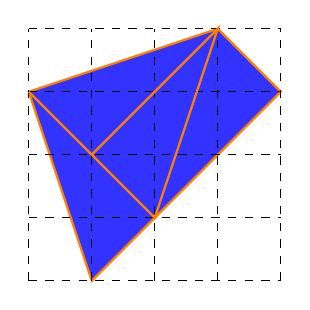
\begin{tikzpicture}[scale=0.8]
		\filldraw [color=blue!80] (1,0)--(4,3)--(3,4)--(0,3)--cycle;
		\draw [thick,color=orange]  (1,0)--(4,3)--(3,4)--(0,3)--cycle;
		\draw [dashed] (0,0) grid (4,4);
		\draw [thick, color=orange] (0,3)--(2,1)--(3,4)--(1,2);
	\end{tikzpicture}
\end{center}
$\pmb{5.}$ Trong ống nghiệm người ta nuôi cấy cả \linebreak virus và vi khuẩn, tổng số là $2000$ con. Đầu tiên mỗi con vi khuẩn tiêu diệt $3$ con virus. Sau đó mỗi con virus còn lại lại tiêu diệt $2$ con vi khuẩn. Tiếp theo mỗi con vi khuẩn còn lại lại tiêu diệt $3$ con virus. Trò ``ăn miếng trả miếng" cứ thế tiếp diễn cho đến khi quân số hai bên trở nên bằng nhau. Hỏi lúc đó mỗi loài còn lại bao nhiêu con?
\begin{figure}[H]
	\centering
	\vspace*{-5pt}
	\captionsetup{labelformat= empty, justification=centering}
	\includegraphics[width=0.6\linewidth]{b55}
	\vspace*{-10pt}
\end{figure}
\textit{Lời giải.} Chúng ta sẽ giải bài toán ``từ dưới lên", có nghĩa là bắt đầu từ thời điểm trong ống nghiệm số virus và số vi khuẩn bằng nhau gồm $M$ con mỗi loài. Một câu hỏi đặt ra: loài nào sẽ giáng đòn cuối cùng? Vì ta chưa biết điều này nên ta sẽ xét $2$ trường hợp.
\vskip 0.1cm
Giả sử vi khuẩn  là loài giáng đòn tiêu diệt cuối cùng. Khi đó trước đòn này có $M+3M=4M$ con virus. Trước đòn cuối này có $M+2\cdot 4M=9M$ con vi khuẩn. Và trước đòn tiêu diệt của $9M$ con vi khuẩn này có $4M+3\cdot9M= 31M$ con virus. Nhận xét thấy theo đề bài, các con vi khuẩn xông vào trận chiến đầu tiên, hơn nữa chúng tấn công vào lũ virus không ít hơn $2$ lượt. Vì thế,  thời điểm khi có $9M$ con vi khuẩn và $31M$ con virus được hoàn toàn có thể tính được là thời điểm ban đầu. Khi đó tổng số các con vi sinh vật này là $9M+31M=40M$. Theo điều kiện ta có $40M=2000$, suy ra $M=50$. Như vậy trong trường hợp này còn lại $50$ con virus và $50$ con vi khuẩn còn sống sót sau một cuộc giao tranh.
\vskip 0.1cm
Nếu thời điểm ban đầu không phải là lúc có $9M$ con vi khuẩn và $31M$ con virus mà cuộc trao đổi ``lịch sự" còn diễn ra lâu hơn, ta có thể thấy dẫn đến mâu thuẫn (nếu xét các phương án thay vì $(9M,31M)$ là các cặp $(71M,244M)$ hoặc $(559M,1921M)$), liên quan tới tính chia hết hoặc điều kiện $M \ge 1$. 
\vskip 0.1cm
Tương tự, nếu xét khả năng loài virus tung ra cú tấn công cuối cùng ta cũng nhận được mâu thuẫn với điều kiện của bài toán.
\vskip 0.1cm
Kết luận: sau một trận giao tranh ác liệt, trong ống nghiệm còn lại $50$ con virus và $50$ con vi khuẩn.
\vskip 0.1cm
$\pmb{6.}$ Các số tự nhiên từ $1$ tới $100$ được viết theo thứ tự liên tiếp. Có $25$ số trong số đó bị gạch đi. Liệu có thể luôn gạch thêm $25$ số, sao cho tổng $50$ số đã bị gạch đi bằng tổng của $50$ số chưa bị gạch hay không?
\vskip 0.1cm
\textit{Lời giải.} Câu trả lời là có thể gạch thêm $25$ số thỏa mãn yêu cầu đề bài. Ta làm như sau.
\vskip 0.1cm
Một trăm số tự nhiên từ $1$ tới $100$ được chia thành $50$ cặp, mỗi cặp có tổng bằng $101$. Ta gọi những cặp này là cặp đôi ``hoàn hảo". Giả sử trong $25$ số bị gạch đi có đúng $k$ cặp ``hoàn hảo", thì còn lại là $25-2k$ số bị lẻ cặp. Ta thêm vào $25-2k$ số lẻ cặp này $25-2k$ số cùng cặp đôi ``hoàn hảo" với nó (bổ sung cho thành đủ cặp) rồi gạch đi toàn bộ các số này. Số các số còn lại là $75 – (25-2k)=50+2k$ và đều có thể xếp thành cặp ``hoàn hảo" (do các số trong cặp lẻ với $25$ số bị xóa ban đầu cũng đã bị xóa nốt). Số các cặp ``hoàn hảo" đã xóa đi là $k+(25-2k)=25-k$. Như vậy số các cặp còn lại là $25+k$. Giờ ta xóa đi nốt $k$ cặp bất kỳ trong $25+k$ cặp còn lại. Như vậy ta còn có đúng $25$ cặp ``hoàn hảo" còn lại chưa bị xóa và  tổng của chúng bằng $ 101 \cdot 25$, đúng bằng $\frac{1}{2}$ tổng các số tự nhiên từ $1$ tới $100$.
\end{multicols}
\newpage
\thispagestyle{toancuabinone}
\blfootnote{\color{toancuabi}$^1$Ottawa, Ontario, Canada.}
\begingroup
\AddToShipoutPicture*{\put(60,733){\includegraphics[width=17.2cm]{../mathc.pdf}}}
%\AddToShipoutPicture*{\put(-2,733){\includegraphics[width=17.2cm]{../mathl.pdf}}} 
\AddToShipoutPicture*{\put(68,640){\includegraphics[scale=1]{../tieude3.pdf}}} 
\centering
\endgroup

\vspace*{75pt}

\begin{multicols}{2}
	\textbf{\color{toancuabi}If this is true then $\pmb{\ldots}$, if this is false then~$\pmb{\ldots}$}
	
	\vspace*{5pt}
	\PIbox{{\color{toancuabi}\textbf{Example} (Who is younger?)}
		\vskip 0.15cm
		A brother and a sister were once asked who was younger. ``I am older," said the brother. ``I am younger," said the sister.
		\vskip 0.15cm
		Now, if you knew that \textit{at least one of them lied,}
		then who was younger?
		\begin{figure}[H]
			\centering
			\vspace*{-5pt}
			\captionsetup{labelformat= empty, justification=centering}
			\includegraphics[width=1\linewidth]{Pi5_ToanTA_Hinh1}
%			\vspace*{-15pt}
		\end{figure}}
	\vskip 0.2cm
	There are two different approaches to this problem.
	\vskip 0.15cm
	\textit{Solution} $1$. The first one is to \textit{evaluate all possible truths} and see which one matches the given conditions.
	There are two cases: the brother was younger, or the sister was younger.  
	\vskip 0.15cm	
	If the brother was younger, then the brother lied, and so did the sister.
	If the sister was younger, then both of them told the truth, which would not be possible.
	\vskip 0.15cm	
	Thus, the brother was younger, and they both lied.
	\vskip 0.15cm
	\textit{Solution} $2$. Now, the second approach is to \textit{evaluate all possible assumptions}, in this case whether the brother (and then the sister) told the truth.
	\vskip 0.15cm
	If the brother told the truth, then the sister did too, and
	this contradicts the condition that at least one of them lied.
	If the brother lied, then the sister lied too, so
	this satisfies the condition, and therefore it is the correct one.
	\vskip 0.15cm		
	Thus, the brother was younger, and they both lied.
	\vskip 0.2cm
	\PIbox{{\color{toancuabi}\textbf{Example} (How can they see each other?)}
	\vskip 0.15cm
	Two camels were facing in opposite directions.
	One was facing due east and the other one was facing due west.
	How can they manage to see each other, without walking, turning around, or even moving their heads?
	\begin{figure}[H]
		\centering
		\vspace*{-5pt}
		\captionsetup{labelformat= empty, justification=centering}
		\includegraphics[width=1\linewidth]{Pi5_ToanTA_Hinh2}
		\vspace*{-15pt}
	\end{figure}}
	
	\vspace*{5pt}	
	\textit{Solution.}
	The two camels were \textit{facing each other} the whole time, hence facing in opposite directions.
	\vskip 0.15cm
	\columnbreak
	\textbf{\color{toancuabi}How not to die}
	\vskip 0.1cm
	\PIbox{{\color{toancuabi}\textbf{Example} (Defeat King Haggard)}
		\vskip 0.1cm
		There are ten wells in the far, far away Dark Forest.
		The wells are marked by signs with number from $1$ to $10$.
		The water from these wells look and taste like normal water;
		however, they were all poisoned.
		The only known antidote is water from a higher-numbered well.
		(\textit{For example, if you had a sip of water from the well number $6$,
		you could save yourself by drinking from the well $7$, $8$, $9$, or $10$.})
		\vskip 0.1cm
		Unfortunately, there is no antidote for the water from the $10^{\text{th}}$ well.
		While the first nine wells can be easily visited,
		the $10^{\text{th}}$ well is inside the castle of King Haggard, the ruler of the Dark Forest.
		\vskip 0.1cm
		Prince Martin challenged the King to a duel:
		\textit{Each participant should drink a cup of water offered by the opponent.}
		Of course, King Haggard agreed. His plan was to use his $10^{\text{th}}$ well;
		because the water from this well help him survive any drink offered by Prince Martin,
		and it will definitely kill the prince.
		\vskip 0.1cm
		The duel took place as planned. Each participant drank the cup of water offered by the opponent.
		Everybody is surprised and delighted to see that Prince Martin lived and King Haggard died.
		\vskip 0.1cm
		How did this happen?
		\begin{figure}[H]
			\centering
			\vspace*{-5pt}
			\captionsetup{labelformat= empty, justification=centering}
			\includegraphics[width=1\linewidth]{Pi5_ToanTA_Hinh3}
			\vspace*{-15pt}
		\end{figure}}
		\textit{Solution.} 
		Prince Martin \textit{gave King Haggard a drink of clear water.}
		Thus instead of curing him, the water from the $10^{\textrm{th}}$ well he drank then poisoned him.
		Prince Martin, before the duel, drank some water from any of the wells with a number smaller than $10$.
		Therefore \textit{Haggard's cup of water from the $10^{\text{th}}$ well actually cured Prince Martin.}
	\vskip 0.1cm
	\PIbox{
	\textbf{\color{toancuabi}Từ vựng}
	\vskip 0.1cm
	(Quy ước viết tắt: dt=danh từ, tt= tính từ, đt=động từ, ph.t=phó từ.)\vskip 0.1cm 
	\vskip 0.1cm
	{\color{toancuabi}antidote:} (dt)  thuốc giải độc.\vskip 0.1cm 
	{\color{toancuabi}approach:} (dt) tiếp cận.\vskip 0.1cm 
	{\color{toancuabi}assumption:} (dt) giả thiết.\vskip 0.1cm 
	{\color{toancuabi}camel:} (dt) con lạc đà.\vskip 0.1cm 
	{\color{toancuabi}castle:} (dt) lâu đài.\vskip 0.1cm 
	{\color{toancuabi}condition:} (dt) điều kiện.\vskip 0.1cm 
	{\color{toancuabi}cure:} (đt) chữa, chữa khỏi bệnh.\vskip 0.1cm 
	{\color{toancuabi}defeat:} (đt) đánh bại.\vskip 0.1cm 
	{\color{toancuabi}delighted:} (tt) vui sướng, vui mừng.\vskip 0.1cm 
	{\color{toancuabi}direction:} (dt) hướng.\vskip 0.1cm 
	{\color{toancuabi}due east:} (dt) hướng chính Đông.\vskip 0.1cm 
	{\color{toancuabi}due west:} (dt) hướng chính Tây.\vskip 0.1cm 
	{\color{toancuabi}duel:} (dt) cuộc đấu tay đôi.\vskip 0.1cm 
	{\color{toancuabi}evaluate:} (đt) ước lượng, định giá.\vskip 0.1cm 
	{\color{toancuabi}face:} (đt) nhìn về, hướng về.\vskip 0.1cm 
	{\color{toancuabi}lie:} (đt) nói dối.\vskip 0.1cm 
	{\color{toancuabi}manage:} (đt) xoay sở được, tìm được cách.\vskip 0.1cm 
	{\color{toancuabi}mark:} (đt) đánh dấu.\vskip 0.1cm 
	{\color{toancuabi}match:} (đt) xứng, hợp.\vskip 0.1cm 
	{\color{toancuabi}plan:} (dt) kế hoạch.\vskip 0.1cm 
	{\color{toancuabi}poison:} (đt) làm nhiễm độc.\vskip 0.1cm 
	{\color{toancuabi}ruler:} (dt) người thống trị.\vskip 0.1cm 
	{\color{toancuabi}sign:} (dt) dấu, dấu hiệu.\vskip 0.1cm 
	{\color{toancuabi}sip:} (dt) một ngụm, một hớp.\vskip 0.1cm 
	{\color{toancuabi}surprise:} (đt) ngạc nhiên.\vskip 0.1cm 
	{\color{toancuabi}survive:} (đt) sống sót.\vskip 0.1cm 
	{\color{toancuabi}well:} (dt) cái giếng.	
	}	
\end{multicols}
